\section{Architecture}
\label{sec:architecture}
\writer{Albert and Monica}
The architecture of this \epns has been designed as modular, meaning that the system is divided in different components which are connected through interfaces. In this way, components are independent of each other and can be developed by different members of the team. In addition, the modular design is an advantage for easily testing each component as well as the entire system in a hierarchical structure.     

\begin{figure}[htp]
\begin{center}
  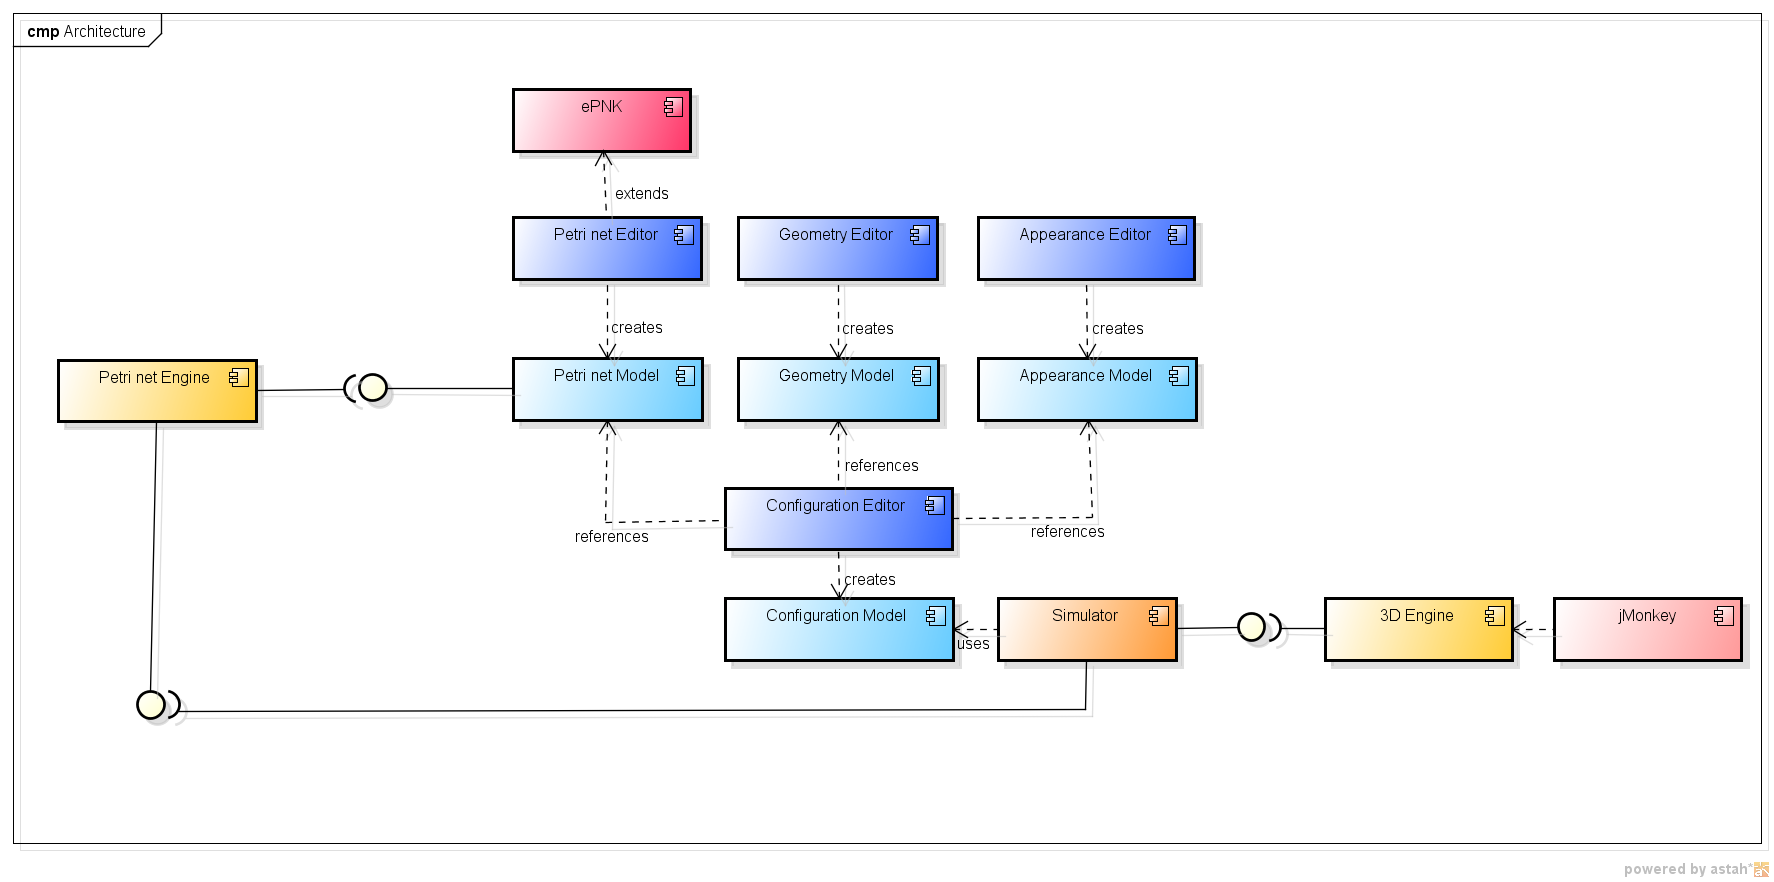
\includegraphics[width=0.8\textwidth]{image/cd-architecture.png}
  \caption{Architecture of the System}
  \label{fig:architecture}
\end{center}
\end{figure}

\begin{figure}[htp]
\begin{center}
  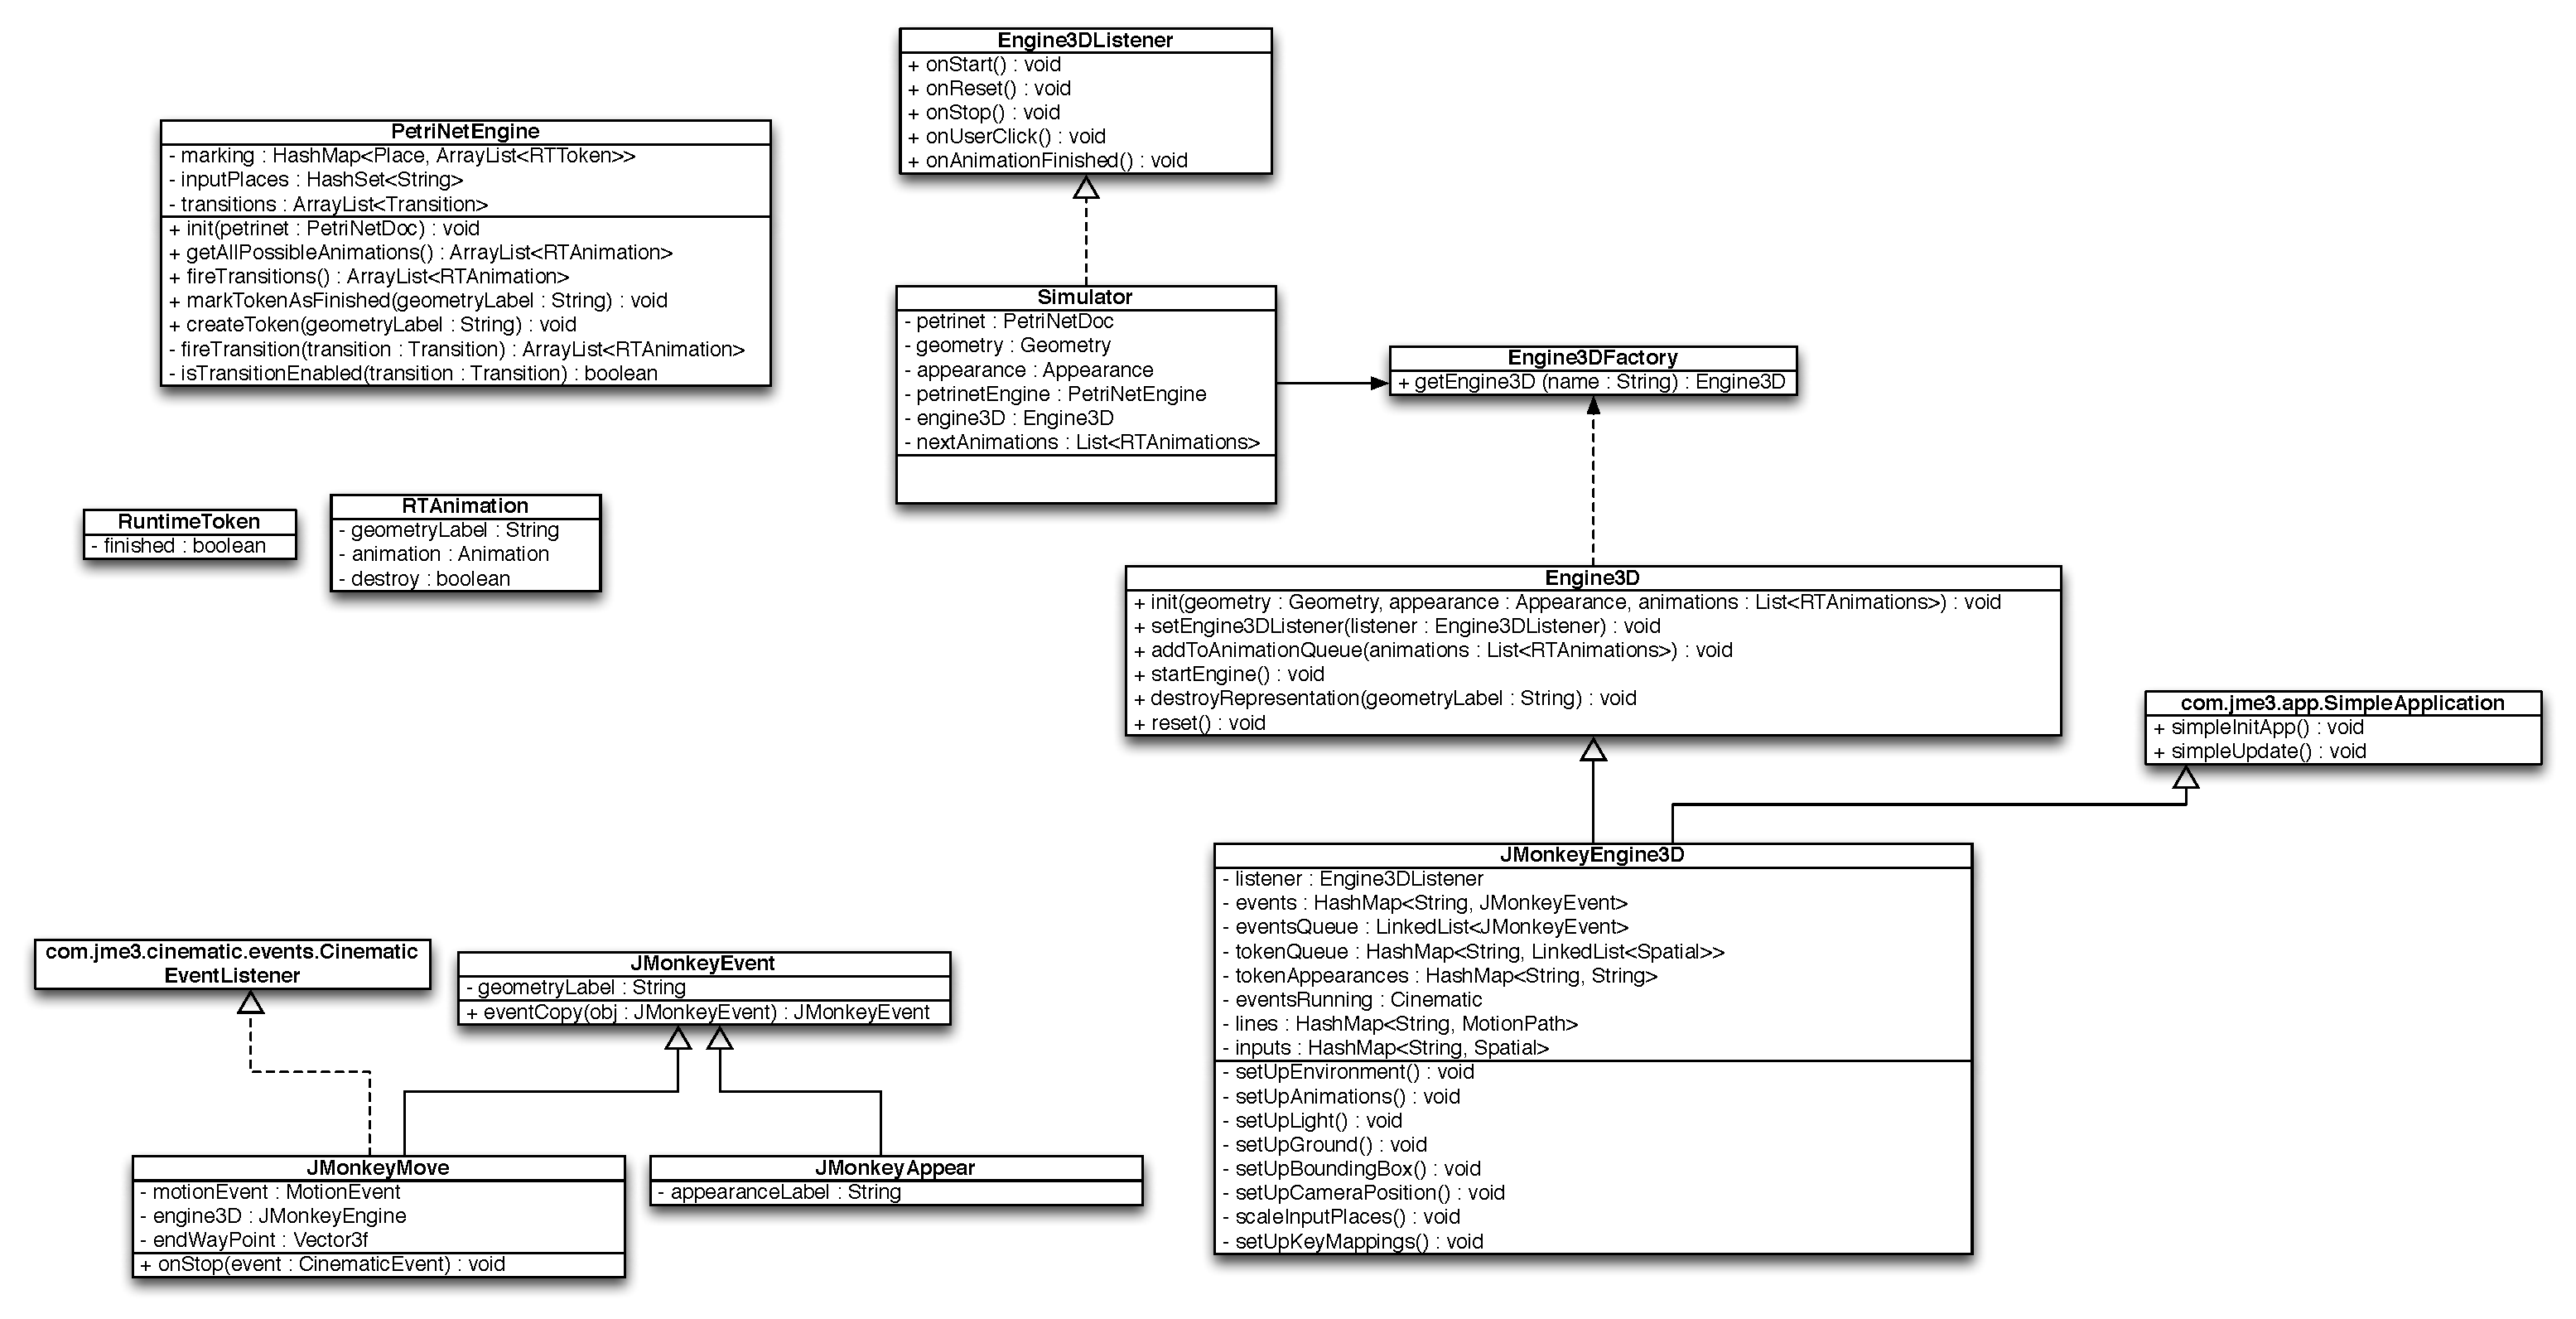
\includegraphics[width=0.8\textwidth]{image/domain.pdf}
  \caption{Class diagram of the system}
  \label{fig:class-diagram}
\end{center}
\end{figure}


\subsection{Petri net editor}
\writer{Albert}

The Petri net editor is a component which consists of an extension of the ePNK editor. It contains all the functionality that ePNK provides and also adds the features described previously in this document, and that can be summarized in Figure \ref{fig:uml-petrinet-editor}. Its actual implementation is shown in Figure \ref{fig:petri-net-domain-model}.

\begin{figure}[htp]
\begin{center}
  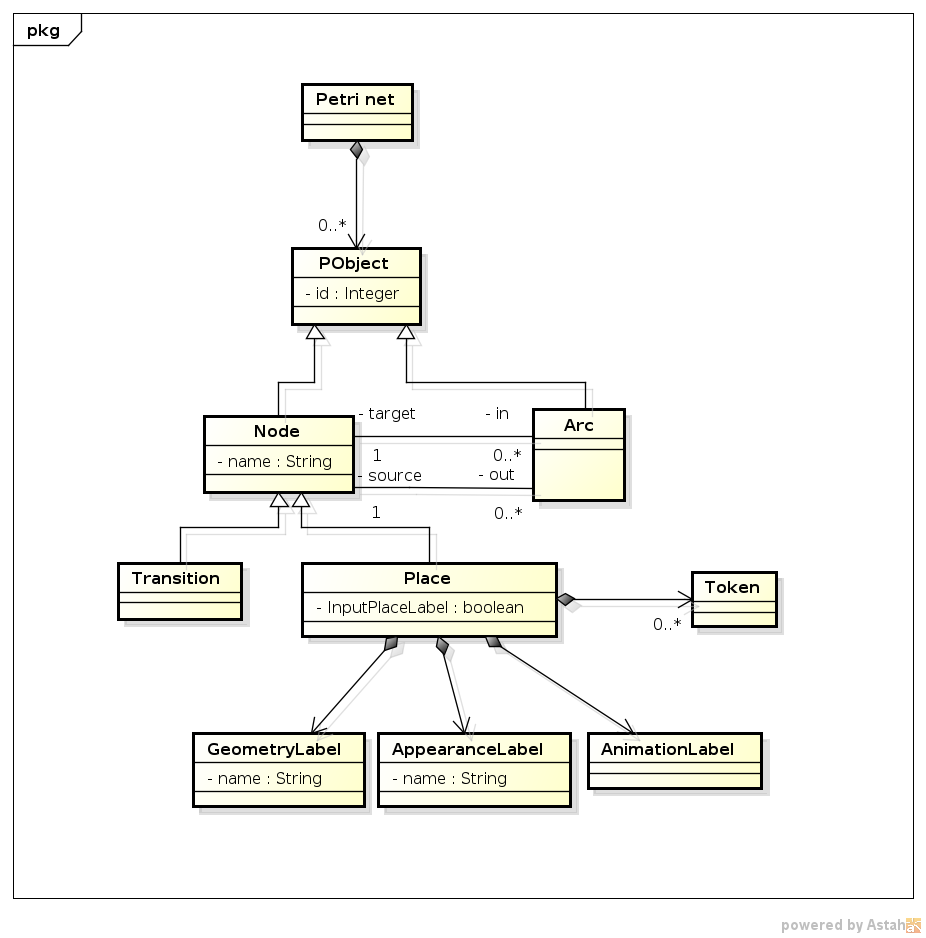
\includegraphics[width=0.8\textwidth]{image/petrinet_uml.png}
  \caption{UML for the Petri net Editor}
  \label{fig:uml-petrinet-editor}
\end{center}
\end{figure}

\begin{figure}[htp]
\begin{center}
  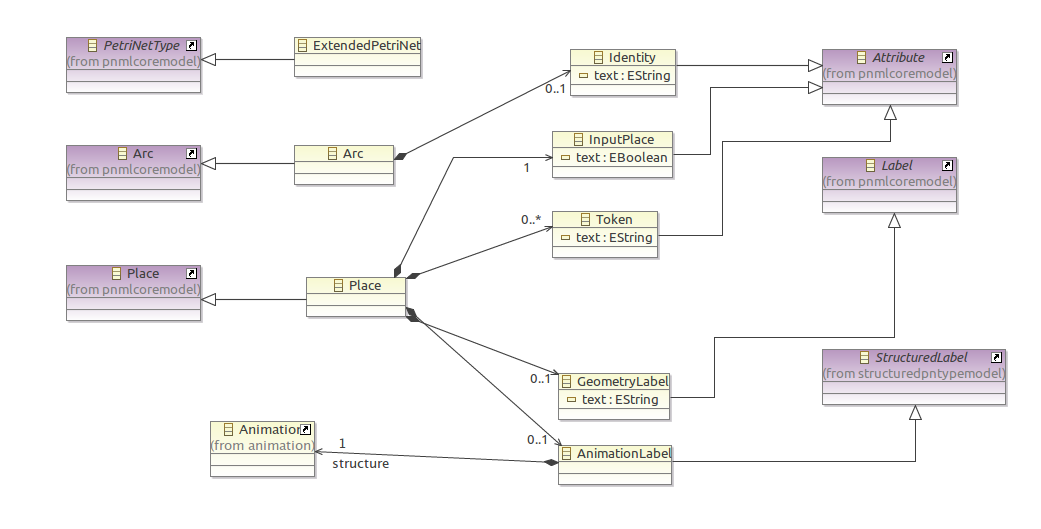
\includegraphics[width=0.8\textwidth]{image/petrinet_editor_domain.png}
  \caption{Petri net editor domain model}
  \label{fig:petri-net-domain-model}
\end{center}
\end{figure}

\subsubsection{Petri net editor classes}

A description of the classes shown in Figure \ref{fig:petri-net-domain-model} is provided.

\paragraph{Place}

The class Place extends from Place in the \textit{pnmlcoremodel}, and contains the following attributes:

\begin{itemize}
	\item \textbf{Token}
	\item \textbf{AppearanceLabel}: an ePNK string label to indicate the shape and texture of the Place.
	\item \textbf{InputPlaceLabel}: an ePNK boolean attribute to indicate if the place is interactive for the user or not (if tokens can be added in runtime by the user).
	\item \textbf{GeometryLabel}
	\item \textbf{AnimationLabel}
\end{itemize}

\paragraph{Arc}

\subsection{Geometry editor}
\label{sec:arch-geometry}
\writer{Mikko}

The Geometry editor is the component used to define lines and points in a two dimensional plane which will then define the location and overall shape of the visualized simulation. Figure \ref{fig:model-geometry} describes the geometry model used by the Geometry Editor.

\begin{figure}[htp]
\begin{center}
  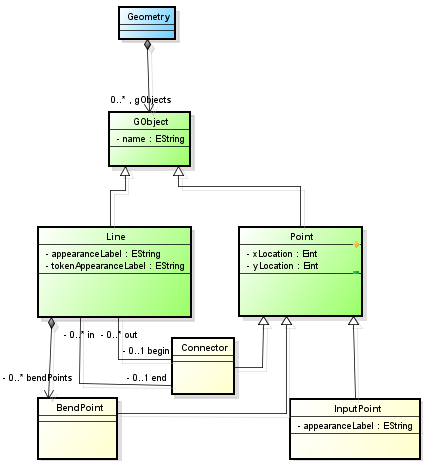
\includegraphics[width=0.8\textwidth]{image/geometry_diagram.png}
  \caption{Geometry domain model}
  \label{fig:model-geometry}
\end{center}
\end{figure}

\paragraph{Geometry}
The Geometry class is an abstract definition of a geometry object.

\paragraph{GObject}
The GObject is a geometry object, which can be either a line or a point. It has attribute \textbf{name}. It is used to name individual geometry objects, so that user can easily tell them apart. Furthermore, it is used as an identifier for all geometry objects.

\paragraph{Point}
Point is a location in the two dimensional plane. It has attributes \textbf{xLocation} and \textbf{yLocation} which refer to the horizontal and vertical coordinates respectively.

\paragraph{InputPoint}
Class InputPoint refers to objects that will be clickable for the user in the 3D simulation. The\textbf{AppearanceLabel} attribute is used to identify the 3D appearance of an InputPoint, such as traffic light, tree, planet etc, within the simulation.

\paragraph{Connector}
Class Connector is either the beginning or the ending parametric point of a line. Therefore, lines that end at a Connector are \textbf{in} and lines that start from a Connector are \textbf{out}.

\paragraph{BendPoint}
Class BendPoint is the type of parametric point that defines the curvature of the line.

\paragraph{Line}
Class Line is a parametric curve in the two dimensional plane. The line begins at a point location \textbf{begin} and it ends at a point location \textbf{end}. A \textbf{BendPoint} is a point location which defines in a parametric way the curvature of the line, unless it doesn't have one, thus the line would be straight. The\textbf{AppearanceLabel} attribute is used to define the 3D shape of the line within the simulation. The appearance will be extrapolated along the length of the line, thus the appearance could for instance be track, road, empty space, etc. On the other hand, the \textbf{tokenAppearanceLabel} attribute defines 3D models that are animated along the line. They could be for instance train, bike, space ship, etc.

The geometry editor is initially implemented with Graphical Modeling Framework (GMF). It provides the factory pattern for construction of objects, command pattern for the editing functionality and interfaces for function calls. The implementation is then extended with listeners. The listener notifies the geometry of the changes done to the location of a graphical object in the graphical editor. This information is used to define coordinate locations of geometry objects. Furthermore, the visualization of lines, or as they are called in GMF- connections, in the graphical editor is changed to that of catmull-rom curves. 






\subsection{Appearance editor}
\subsection{Configuration editor}
\writer{Monica}

The Configuration Editor is the component which allows the user to create a link between all the models that have been previously created by using the other editors. The editor can be used by both technical and non-technical users since its main functionality is connecting the Petri net, the Geometry and the Appearance models. 

Figure \ref{fig:uml-configuration-editor} shows the model behind the Configuration Editor. 

\begin{figure}[htp]
\begin{center}
  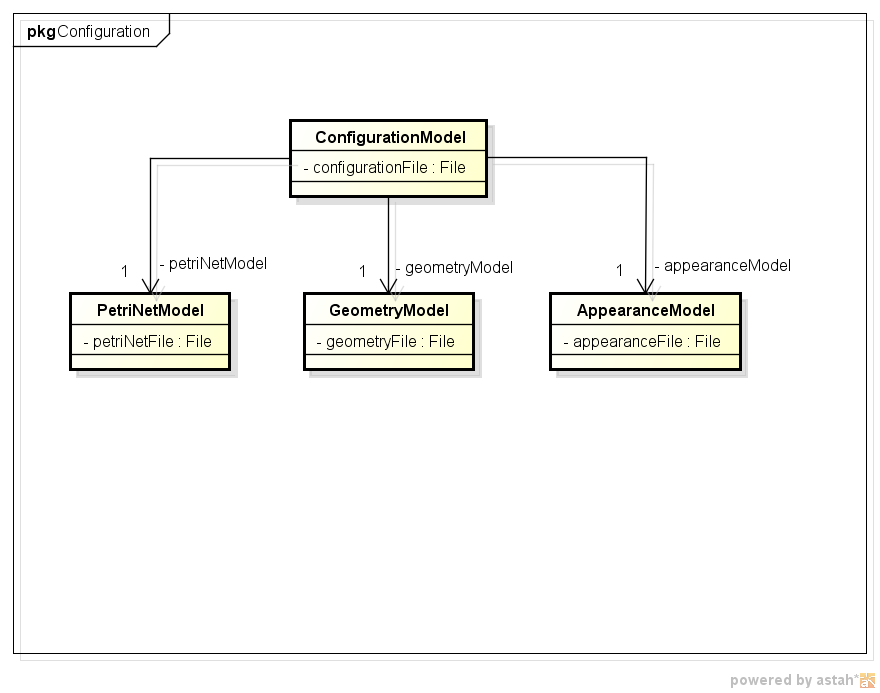
\includegraphics[width=0.8\textwidth]{image/configuration-model.png}
  \caption{UML for the Configuration Editor}
  \label{fig:uml-configuration-editor}
\end{center}
\end{figure}

\subsubsection{Configuration editor classes}

Next, a more detailed description of the model is provided.

\paragraph{ConfigurationModel}

The ConfigurationModel class has only one attribute, \textbf{configurationFile}, of type File, which will include all the information provided by the \textit{PetriNetModel}, \textit{GeometryModel} and \textit{AppearanceModel} objects. 

\paragraph{PetriNetModel}

The PetriNetModel class has only one attribute, \textbf{petriNetFile}, of type File, which represents the output file of the Petri net Editor. This file will include the description of all the objects in the petri net and their attributes. 

\paragraph{GeometryModel}

The GeometryModel class has only one attribute, \textbf{geometryFile}, of type File, which represents the output of the Geometry Editor. This file will include the description of all geometry objects and their attributes.

\paragraph{AppearanceModel}

The AppearanceModel class has only one attribute, \textbf{appearanceFile}, of type File, which represents the output of the Appearance Editor. This file will include the associations between appearance labels of the Petri net objects and their corresponding 3D objects or textures. 


\subsection{Petri net engine}
\subsection{Simulator}
\writer{Albert}

The simulator is the main component of the system, it reads the initial configuration and works as a controller between the Petri net Engine and the 3D Engine.

In order to implement this, we will use the Observer pattern (Figure \ref{fig:observer-pattern}) so that the Simulator can keep track and receive notifications from the 3D engine when some events happen, such as an animation finished or a user interaction.

\begin{figure}[htp]
\begin{center}
  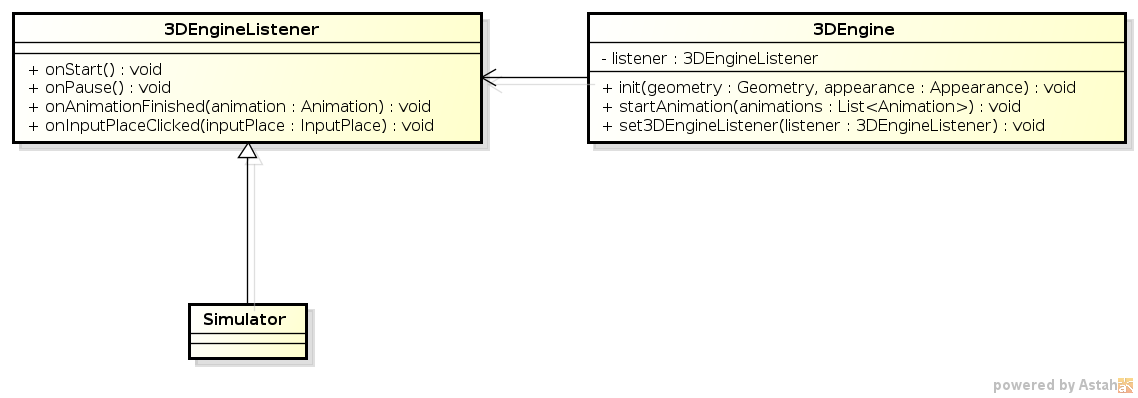
\includegraphics[width=0.8\textwidth]{image/ObserverPattern.png}
  \caption{Simulator with the Observer Pattern}
  \label{fig:observer-pattern}
\end{center}
\end{figure}

Figure \ref{fig:sd-engines} shows the interaction between the three components involved. The simulator starts by reading the configuration, and initializing the Petri net engine with the initial Petri net model as well as the 3D engine with the geometry and the appearance models. 

\begin{figure}[htp]
\begin{center}
  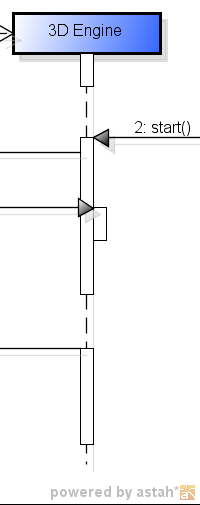
\includegraphics[width=0.8\textwidth]{image/sd-engines.png}
  \caption{Sequence diagram of the Simulator, Petri net Engine and 3D engine}
  \label{fig:sd-engines}
\end{center}
\end{figure}

Then, the 3D engine tells the Simulator that it has received a \textit{start simulation} input from the user, and thus, awaits for new animations to be played. The simulator asks the Petri net engine to fire transitions and to give back the next sequence of animations to be played by the 3D engine.
\subsection{3D Engine}
\subsection{The jMonkeyEngine}
\writer{Anders, Albert}

The interface that described in Section~\ref{sec:3d-engine} will be implemented using jMonkey library. In the following, the implementation of the interface will be described.

\textbf{init(Geometry geometry, Appearance appearance)}
The initialization will put all information about the geometry and appearance into a list of SObjects. An SObject is a line segment, or using Petri Net terms: two transitions and a place. This list of SObjects is then used to set up the animations that will be playable in the simulation. The animations are created using the MotionPath and MotionEvent classes inherited from jMonkey. For each SObject, a MotionPath is created using the points that make up the line segement; this could be a beginning point, a few bend points and an end point. The MotionPath is then used to set up the MotionEvent, which besides needing a MotionPath, also needs some geometry, which in this case will be a shape defined by the SObject. The shape will be the shape of the token on the line segment. All tokens have need to be prepared as jMonkey geometries before creating the MotionEvents.

When all animations are set up in a list of MotionEvents, the paths will have their shape applied. This will make the Petri Net visible to the user. It will require stretching and duplication of the shapes and textures. Also, the camera will be positioned and oriented to its default position, and default background geometry will be created.

The simulator will produce a list of animations for jMonkey to play. Animations may be added to this list at any time. When animations finish, jMonkey will tell the simulator. This is the main interaction between the simulator and jMonkey. So when the system allows users to play, pause and reset the simulation, the play and pause will be handled by jMonkey alone. The simulator will need to know when the user resets the simulation, because it needs to tell the Petri Net engine to reset. But most of the time, the simulator will just wait for information about which animations have finished, and pass that on to the Petri Net engine, which in return will tell the simulator which animations jMonkey should play.

\textbf{onStart()}
The MotionEvent system used to set up the animations allows jMonkey to know the status of each animation. When the user opens the simulator, he will need to press play for the animation to begin. This action will cause jMonkey to run the animations that it was instructed to run by the simulator. If the user is pressing play, while the simulation was paused, jMonkey will simply continue playing all the paused MotionEvents.

\textbf{onPause()}
When the user presses pause, jMonkey will find the animations that are currently running, and pause them. The pause function is already integrated in the MotionEvent class.

\textbf{onReset()}
It the simulation is asked to reset, jMonkey will report to the simulator that it needs to reset the Petri Net engine. This is to ensure that the list of animations is correct.

\textbf{onUserClick()}
When a user clicks, a jMonkey listener will pick it up, and the position determined. If the click was on an input place, the name of the input place will be sent to the simulator, which will tell the Petri Net engine. The Petri Net engine will then determine how this affects the logic.

\textbf{animate(List<Animation> animations)}
The animations in the simulator are started according to the current list of animations waiting to be played. If the simulator is running, all animations arriving in the list of animations will be started instantly.

\textbf{onAnimationFinished(Animation animation)}
The simulator needs to know as soon as animations have finished, in order to quickly get the next animation. The state of all animations is checked 60 times per second, and the delay between one animation finishing and the next starting should be low.

\subsubsection{Collision Detection}
\writer{Thibaud}